%%%%%%%%%%%%%%%%%%%%%%%%%%%%%%%%%%%%%%%%%%%%%%%%%%%%%%%%%%%%%%%%%%%%%%%%%%%%%%
%
% Appendix file included in main project file using \input{}
%
% Assumes that LaTeX2e macros and packages defined in cg_comp.sty are
%   available
%
%%%%%%%%%%%%%%%%%%%%%%%%%%%%%%%%%%%%%%%%%%%%%%%%%%%%%%%%%%%%%%%%%%%%%%%%%%%%%%

 \section{Fretting Model\label{app:fret}}

As discussed in \sct{model}, unlike previous studies of guitar intonation and compensation~\cite{ref:byers1996cgi,ref:varieschi2010icf} we have neglected to include a contribution to the incremental change in the length of the fretted string caused by both the depth and the shape of the string under the finger. As the string is initially pressed to the fret, the total length $\mathcal{L}_n$ increases and causes the tension in the string --- which is pinned at the saddle and clamped at the nut --- to increase. As the string is pressed further, does the additional deformation of the string increase its tension (throughout the resonant length $L_n$)? There are at least two purely empirical reasons to doubt this hypothesis. First, we can mark a string (with a fine-point felt pen) above a particular fret and then observe the mark with a magnifying glass. As the string is pressed all the way to the finger board, the mark does not move perceptibly --- it has become \emph{clamped} on the fret. Second, we can use either our ears or a simple tool to measure frequencies~\cite{ref:pgtweb} to listen for a shift as we use different fingers and vary the fretted depth of a string. The apparent modulation is far less than would be obtained by classical vibrato ($\pm15$~cents), so we assume that once the string is minimally fretted the length(s) can be regarded as fixed. (If this were not the case, then fretting by different people or with different fingers, at a single string or with a barre, would cause additional, varying frequency shifts that would be audible and difficult to compensate.)


\begin{figure}
    \centering
    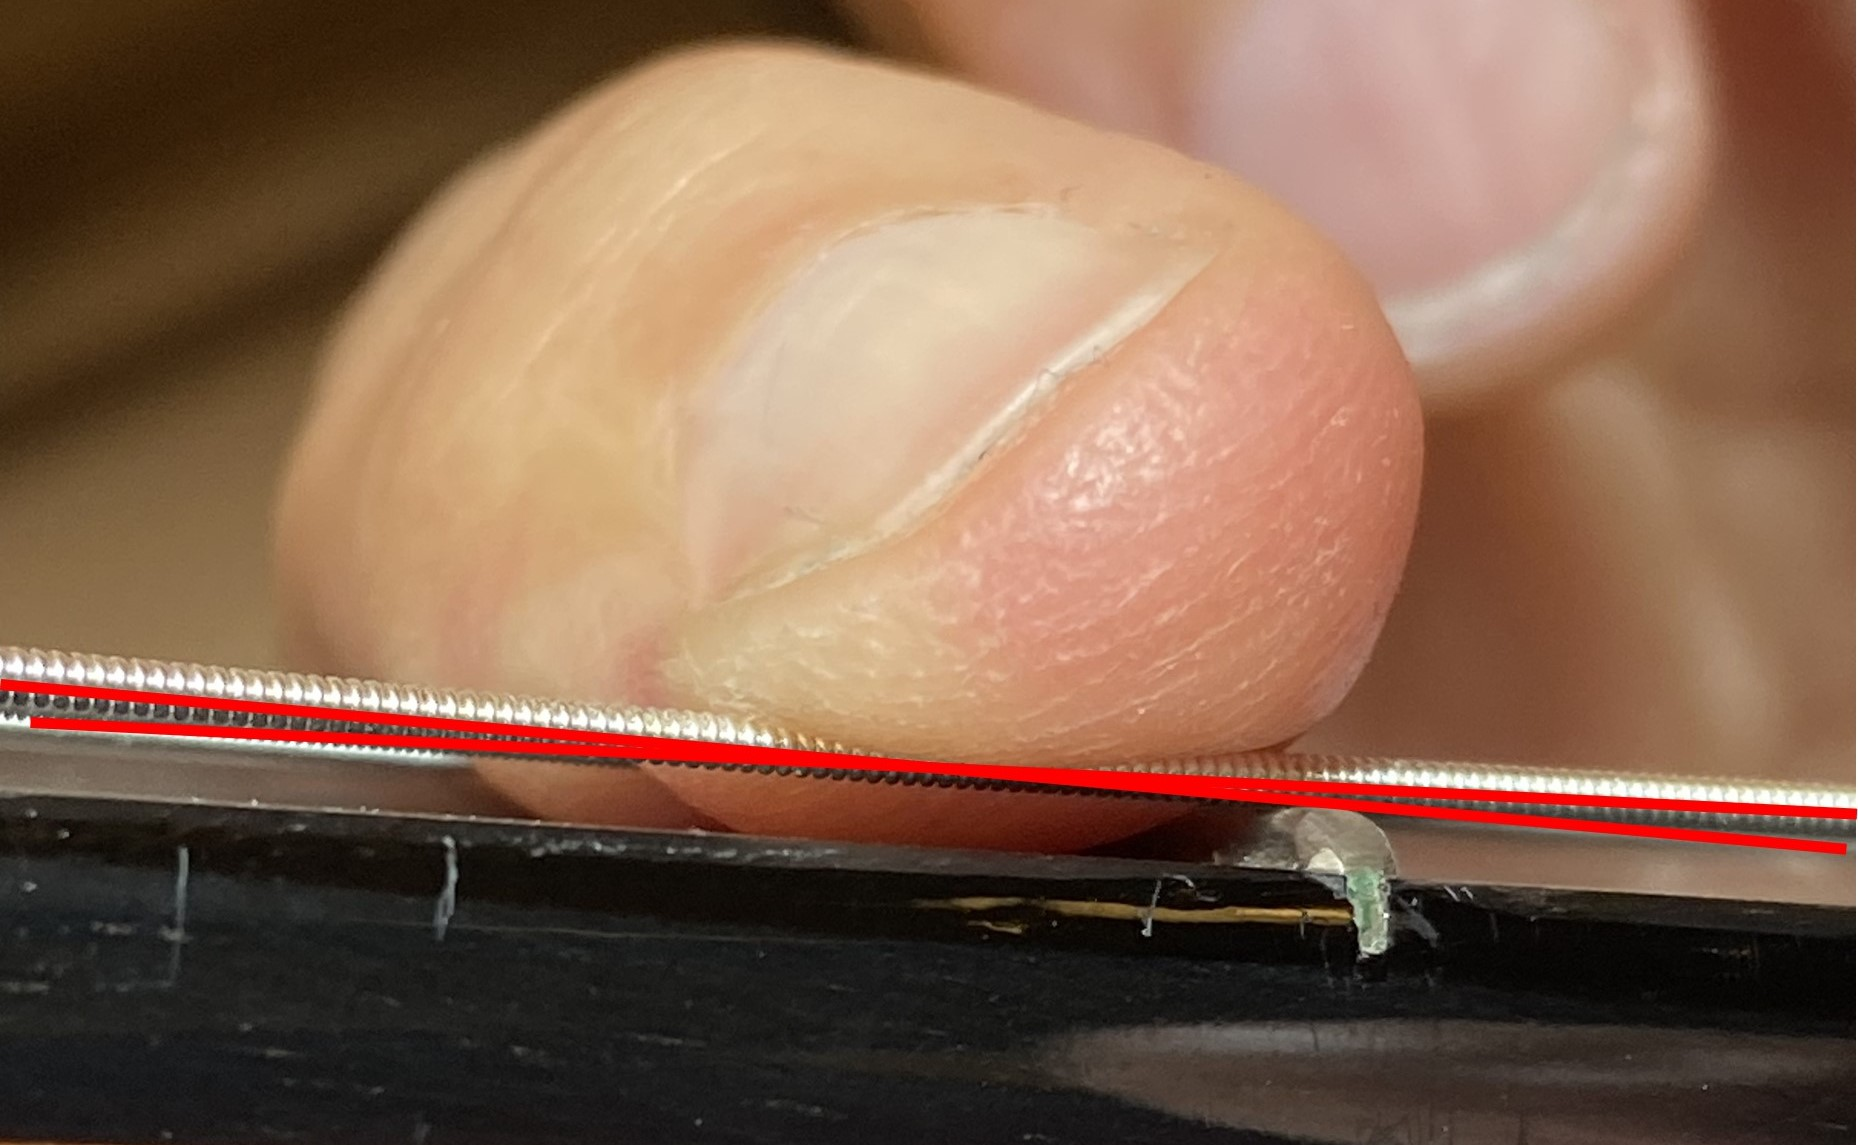
\includegraphics[width=6.0in]{../figures/fretting_photo}
    \caption{\label{fig:fretting_photo} Photo of a wound nylon $E_2$ string clamped at the first fret. The shape of the fretted string can be well approximated by two lines intersecting about 5~mm behind the fret.}
\end{figure}

\begin{figure}
    \centering
    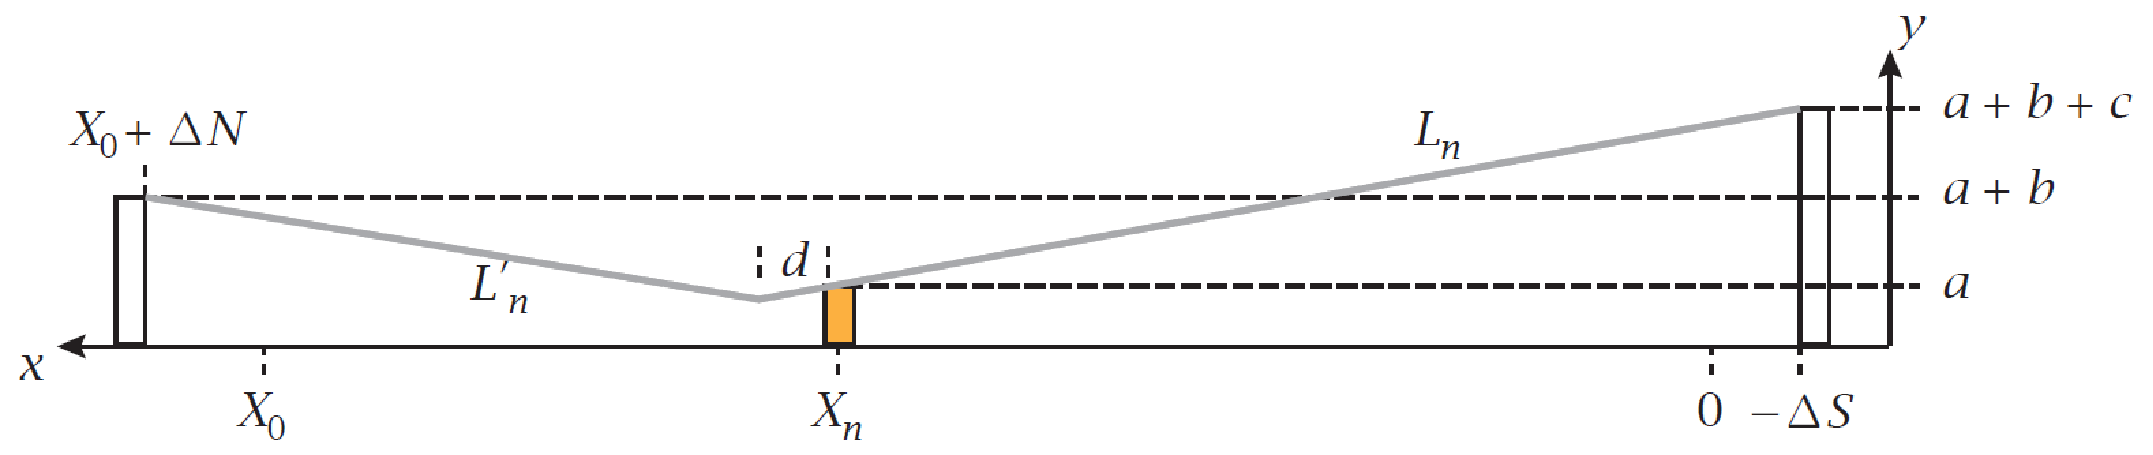
\includegraphics[width=6.0in]{../figures/fretting_schematic}
    \caption{\label{fig:fretting_schematic} A recapitulation of \fig{guitar_schematic} with the addition of a horizontal linear distance $d$ at fret $n$ to represent the slight increase in the distance $L_n^\prime$ caused by a finger.}
\end{figure}

Here we include this concept in a simple way to determine the effect it could have on the frequency shift due to increased string tension. In \fig{fretting_schematic}, we adopt the schematic of the guitar shown in \fig{guitar_schematic}, but we allow a small, horizontal linear section of string with length $d$ to represent the action of the finger. In this case, the resonant length $L_n$ is unaffected, but the remaining string length becomes
 \begin{equation}
L^\prime_n = d + \sqrt{\left(X_0 + \Delta N - X_n - d\right)^2 + b^2} \approx X_0 - X_n + \Delta N + \frac{b^2}{2 \left(X_0 + \Delta N - X_n - d\right)}\, .
 \end{equation}
Roughly speaking, the act of fretting increases the effective value of $b^2$ in $L^\prime_n$ by a factor of $1 + d / (X_0 - X_n)$. We can use this result and \eqn{q_n_approx} to determine the increase in the relative displacement $Q_n$; we find
\begin{equation} \label{eqn:delta_q_n_approx}
    \Delta Q_n \approx \left(\frac{\gamma_n}{\gamma_n - 1}\right)^2 \frac{b^2\, d}{2\, X_0^3}\, .
\end{equation}
The first factor on the \rhs of this expression is well approximated as
\begin{equation}
    \left(\frac{\gamma_n}{\gamma_n - 1}\right)^2 \approx \left[\frac{12}{n\, \ln(2)}\right]^2\, ,
\end{equation}
which is clearly largest at the first fret. When $d > 0$, the corresponding increase in the frequency shift given by \eqn{error_tot} is
\begin{equation} \label{eqn:delta_nu_n_d}
    \Delta \nu_n(d) - \Delta \nu_n(0) = \frac{600}{\ln(2)}\, \left(\frac{\gamma_n}{\gamma_n - 1}\right)^2 \frac{\kappa\, b^2\, d}{2\, X_0^3}\, .
\end{equation}

In \fig{fret_disp}, we plot $Q_1$ for the first fret as a function of the distance parameter $d$. For this example, we have adopted the parameters of a ``no-relief'' Alhambra 8P guitar using normal tension strings. In the worst case, where $d = 1$~cm, $Q_1$ increases by almost $6 \times 10^{-6}$. For a string with $\kappa = 100$, in \fig{fret_shift} we plot $\Delta \nu_n(d) - \Delta \nu_n(0)$ as a function of $d$. Despite this high value of $\kappa$ and the prediction in \fig{fret_shift} that the shift on the first fret could increase by as much as 0.5~cents, our measurements for $\Delta \nu_1$ using the Alhambra 8P guitar and normal tension strings is consistent with the theoretical values using $d = 0$ shown in \fig{shift_alhambra8p_ej45_factory}. Therefore, without a compelling reason to do so, we are reluctant to choose a value of $d$ greater than 0. It is true that we can press the string so hard that it touches the fret board, but the increase in the frequency shift is still less than 1~cent, and this is likely the result of dragging the string over the fret (similar to vibrato) and causing a local change in tension that is inconsistent with the boundary conditions used to derive \eqn{f_m_stiff}.

 \begin{figure}
  \centering
  \begin{subfigure}[b]{0.8\textwidth}
   \centering
   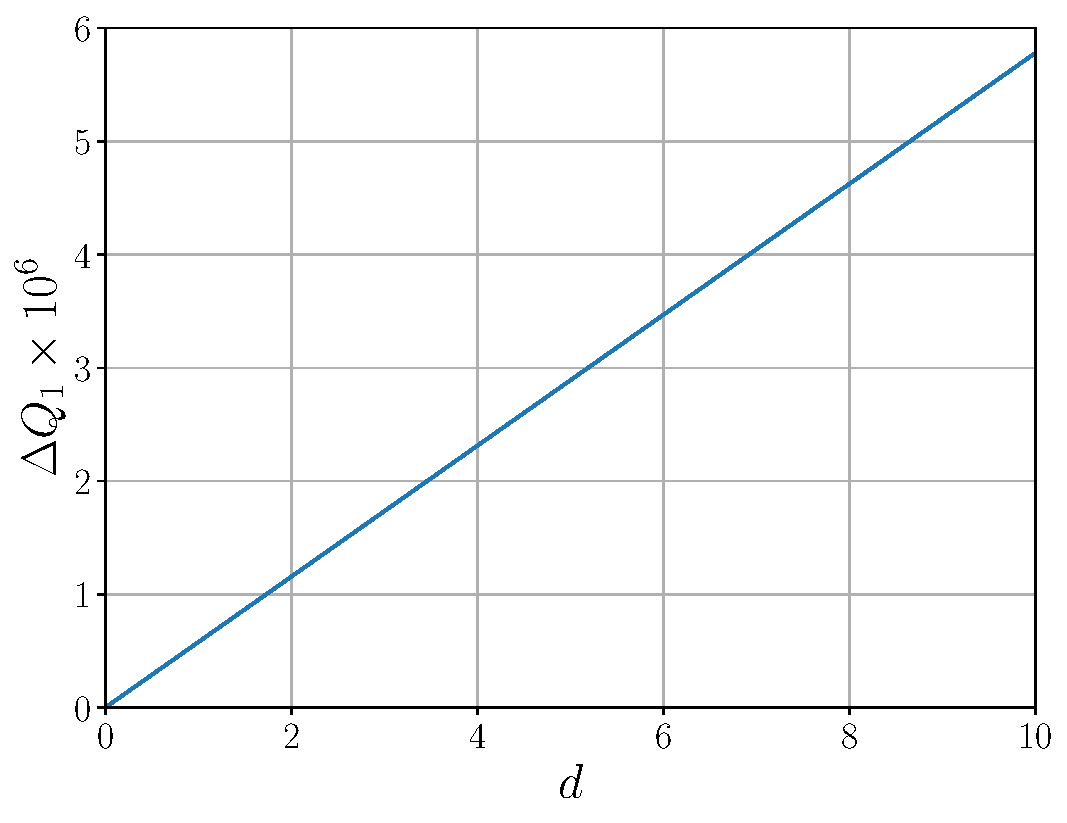
\includegraphics[width=5.0in]{../figures/fret_disp}
   \caption{Relative displacement $Q_1$}
   \label{fig:fret_disp}
  \end{subfigure}
  \par\vspace{0.25in}
  \begin{subfigure}[b]{0.8\textwidth}
   \centering
   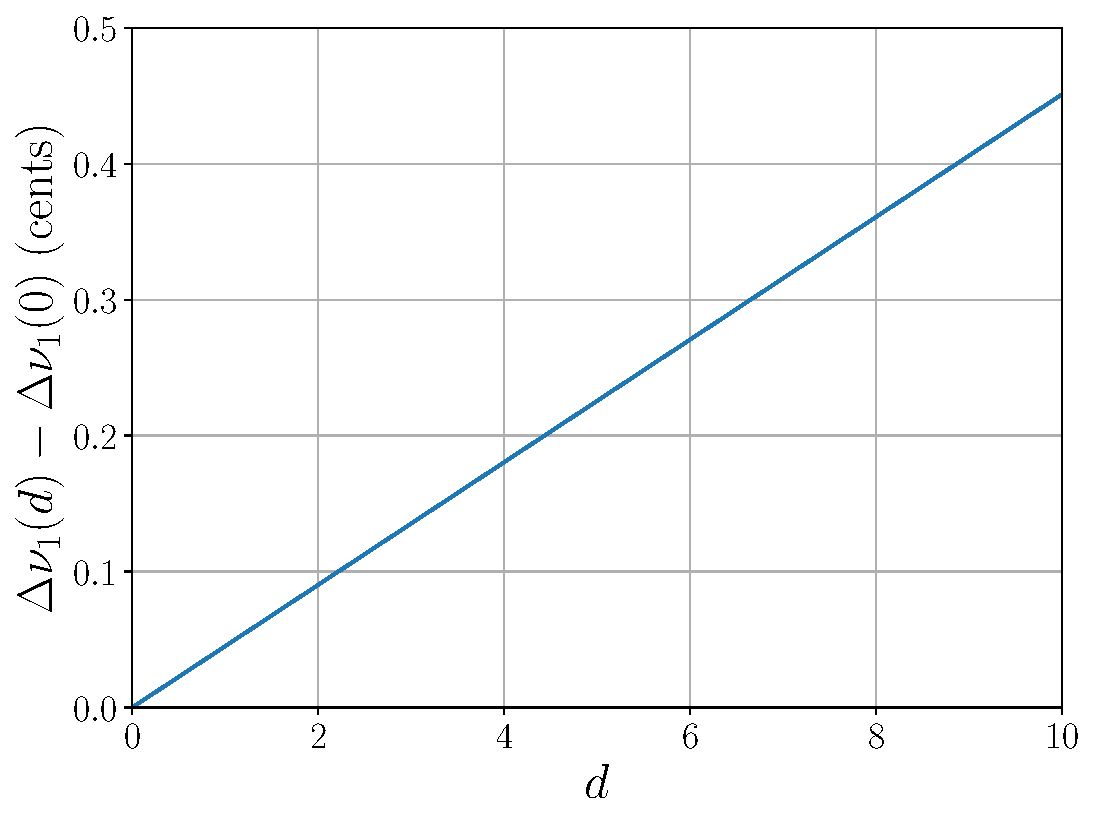
\includegraphics[width=5.0in]{../figures/fret_shift}
   \caption{Additional frequency shift for $\kappa = 100$}
   \label{fig:fret_shift}
  \end{subfigure}
  \caption{\label{fig:fret_model} In (a), we plot the relative displacement $\Delta Q_1$ for the first fret as a function of the fretting distance parameter $d$ using \eqn{delta_q_n_approx}. Here the guitar has the same parameters as the ``no-relief'' Alhambra 8P, with normal tension strings. In (b), we show the additional frequency shift given by \eqn{delta_nu_n_d} at the first fret of a string with $\kappa = 100$ as $d$ increases from 0. For $n > 1$, the relative displacement and additional shift are reduced by a factor of $n^2$.}
 \end{figure}
